\chapter{Einleitung}
Einleitung
Motivation
Referenz auf führere IDPs (Quellen!)
didaktisches Konzept, kurz
Aufbau der Dokumentation, inkl. Benennung wer hat was gemacht (Benotung)

% Keine Beschreibung der Algorithmen an sich!

\chapter{Aufbau der Webanwendungen}
funktionale Beschreibung der Apps
jedes Tab

\section{Algorithmus von Floyd-Warshall}
Da die Implementierung des Floyd-Warshall Algorithmus nicht kompliziert ist, war es wichtig zu zeigen, was genau während dem Ablauf schrittweise passiert. Der Algorithmus wurde in Schritte so unterteilt, dass jeder Schritt eine Verbesserung der Distanz zwischen zwei Knoten darstellt. Um die Verbesserungen anschaulich zu machen, wurde die Adjazenzmatrix implementiert. In jeder Zelle der Adjazenzmatrix wird der aktuelle Distanzwert zwischen zwei entsprechenden Knoten gespeichert. Wenn man die Maus über eine Zelle in der Matrix bewegt, dann wird der Pfad, der diesem Distanzwert entspricht, im Graphen markiert (vgl. Abbildung~\ref{fig:fw-matrix}).

\begin{figure}[h!]
	\centering
	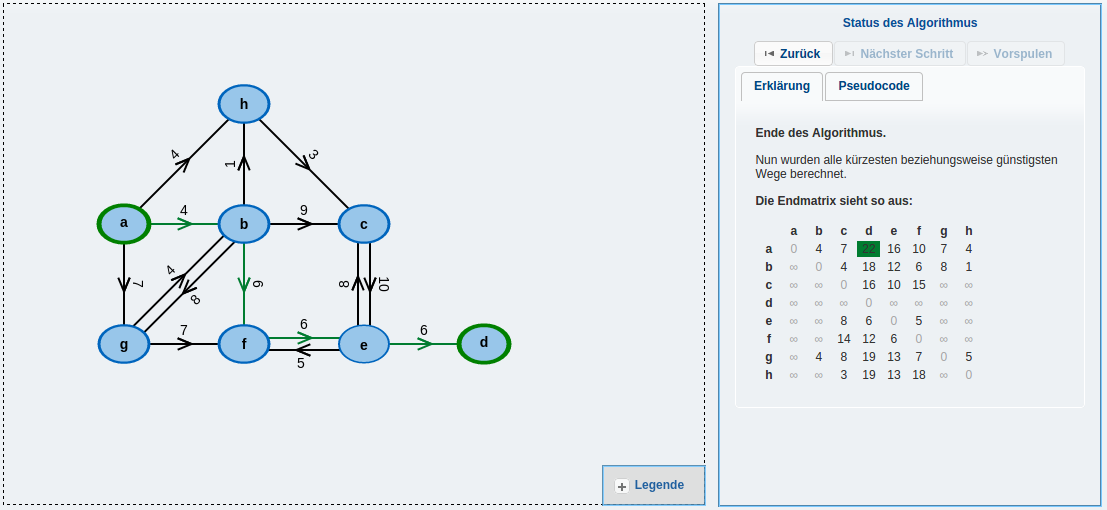
\includegraphics[width=\textwidth]{figures/fw-matrix}
	\caption[Floyd-Warshall Matrix]{Visualisierung des verbesserten Pfades}\label{fig:fw-matrix}
\end{figure}

Die erste Forschungsaufgabe prüft, ob der Nutzer die Logik des Algorithmus verstanden hat. Während des Ablaufs von Floyd-Warshall auf dem bestimmten Graphen werden die Fragen über die vom Algorithmus getroffenen Entscheidungen gestellt.

In der zweiten Forschungsaufgabe soll der Nutzer die fehlende Kantengewichte bestimmen. Ein Teil der Kantenkosten sowie die Adjazenzmatrix sind am Anfang gegeben. Diese Information muss genutzt werden um die fehlende Gewichte zu bestimmen.

\section{Algorithmus von Hierholzer (Mark)}
Beim Algorithmus von Hierholzer war es uns wichtig, die resultierende Eulertour verständlich zu visualisieren. Dazu werden zunächst alle Subtouren in unterschiedlichen Farben dargestellt. Einzelne Subtouren können auf der Ergebnisseite einzeln hervorgehoben werden. Der Benutzer erkennt mittels der Farben außerdem, welcher Teil der Tour aus welcher Subtour stammt. Die Tour kann durch eine Animation (vgl. Abbildung~\ref{fig:hierholzer-animation}) in der richtigen Reihenfolge abgelaufen werden, sodass der Nutzer verifizieren kann, dass es sich wirklich um eine Eulertour handelt.

\begin{figure}[h!]
	\centering
	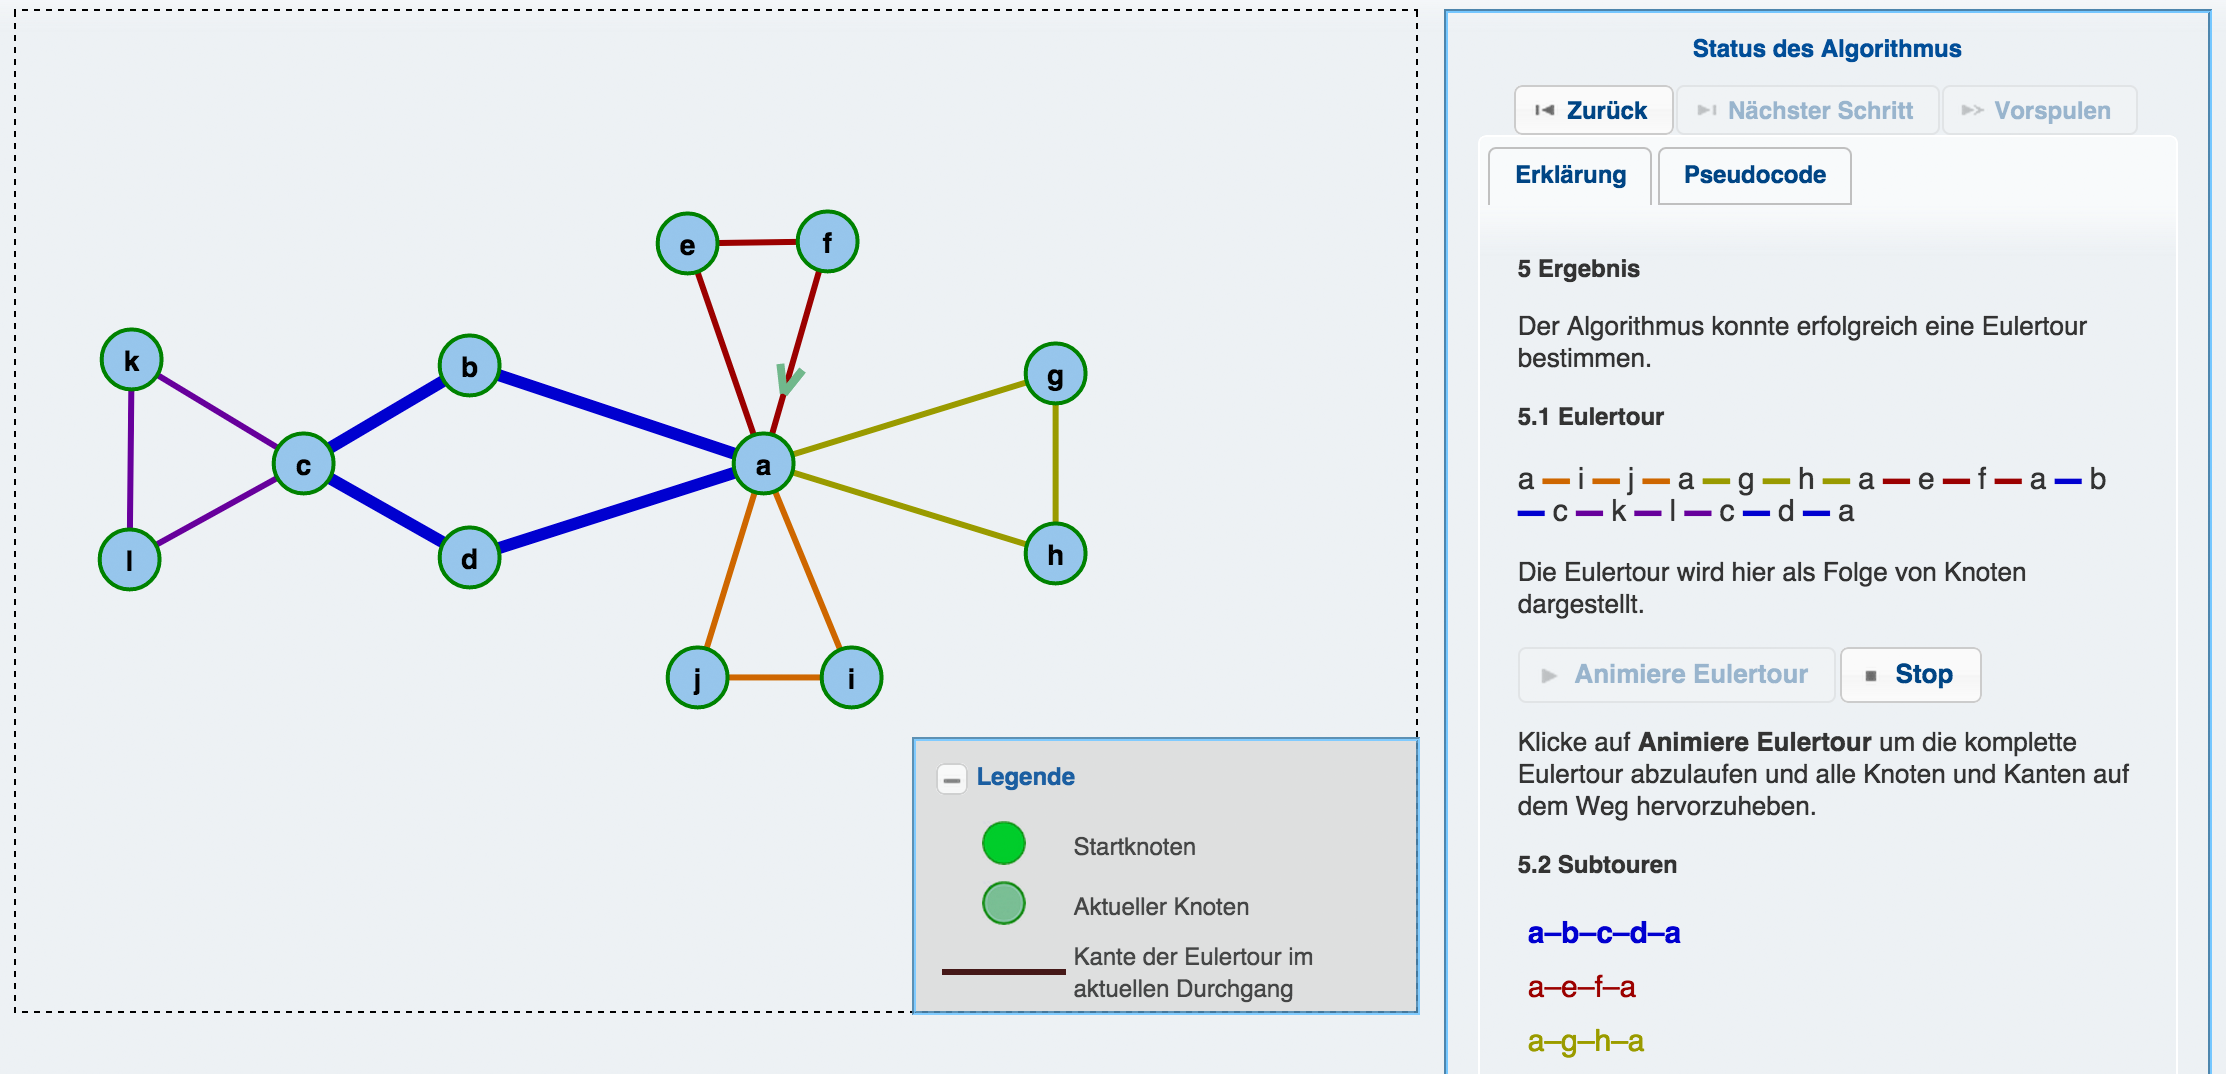
\includegraphics[width=\textwidth]{figures/hierholzer_animation}
	\caption[Eulertour Animation]{Visualisierung der Eulertour mittels Animation}\label{fig:hierholzer-animation}
\end{figure}

Die erste Forschungsaufgabe soll sicherstellen, dass der Nutzer die wichtigsten Abläufe des Algorithmus versteht. Sie behandelt daher im Wesentlichen den Ablauf des Algorithmus, das Konzept des Knotengrads und das Verbinden von Touren.

In einer weiteren Forschungsaufgabe werden die Besonderheiten des Algorithmus bei Anwendung auf einen gerichteten Graphen betrachtet. Der Nutzer betrachtet die geänderten Voraussetzungen, die der Graph erfüllen muss und die veränderte Auswahl der Kanten zur Konstruktion von Subtouren.
     
\section{Algorithmus von Hopcroft und Karp}
Besonderheiten Visualisierung
Forschungsfragen

\section{Ungarische Methode}
Obwohl es mehrere Implementierungen der Ungarischen Methode gibt, die Idee bleibt bei allen gleich. Die Applikation geht nicht tief in die Einzelheiten der konkreten Implementierung, sondern erklärt das generelle Prinzip der Ungarischen Methode. Dafür war der Einsatz des bipartiten gewichteten Graphs notwendig. Als die Ungarische Methode perfektes Matching im bipartiten Graphen sucht, wird eingegebener Graph in der Anwendung bis zum kompletten Graphen vervollständigt falls der Nutzer das nicht gemacht hat. Um die genutzte Begriffe (wie z. B. Matching oder Augmentationsweg) verständlich zu machen, werden unterschiedliche Farben für Knoten und Kanten während des Ablaufs verwendet (vgl. Abbildung~\ref{fig:hungarian-colors}).
\begin{figure}[h!]
	\centering
	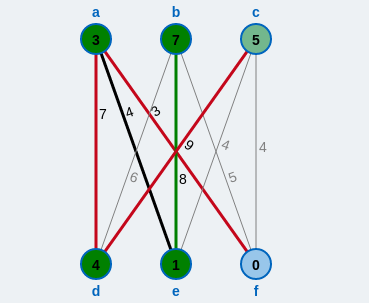
\includegraphics[width=\textwidth]{figures/hungarian-colors}
	\caption[Ungarische Methode]{Augmentationsweg wird rot markiert}\label{fig:hungarian-colors}
\end{figure}

Die erste Forschungsaufgabe prüft, wie gut der Nutzer den Aufbau des Algorithmus verstanden hat. Dazu werden die Fragen während des Ablaufs auf dem beliebigen Graphen gestellt. Der Nutzer muss beantworten, wie der Algorithmus die Markierungen zuweist und welche Schritte macht der Algorithmus als weitere. 

Bei der zweiten Forschungsaufgabe werden auch die Fragen während des Ablaufs der Ungarischen Methode gestellt. Der Graph ist in diesem Fall bestimmt und die Fragen fassen den Aufbau des Augmentationsweges und Gleichheitsgraphs um.

\section{Chinese Postman Problem}
Besonderheiten Visualisierung
Forschungsfragen

\chapter{Implementierung}

\section{Installation (Mark)}
Zur Installation sind keine speziellen Anforderungen zu erfüllen. Die Webapplikationen wurden vollständig mittels HTML5, JavaScript und CSS implementiert, sodass keine zusätzliche serverseitige Software benötigt wird. Zum Aufrufen der Anwendungen wird ein moderner Webbrowser benötigt.

Die Bereitstellung erfolgt über den Online Dienst GitHub, der das verteile Versionskontrollsystem Git benutzt. 
Alle Anwendungen liegen in einem gemeinsamen Repository, welches unter \url{https://github.com/herzog31/adv-graph-algorithms} erreichbar ist. Zur Installation kann man entweder auf der Repository Seite die letzte freigegebene Version (Release) als Zip oder Tar Archiv herunterladen oder die aktuellste Version des Repositories mittels folgendem Befehl in das aktuelle Verzeichnis kopieren.

\begin{figure}[h!]
\begin{lstlisting}[language=Bash]
git clone -b master https://github.com/herzog31/adv-graph-algorithms.git
\end{lstlisting}
\caption[Repository Kopieren]{Befehl zum Kopieren des GitHub Repositories}\label{fig:listing-github}
\end{figure}

Um die Anwendungen als Webanwendungen online bereitzustellen wird ein Webserver benötigt. Hier emfiehlt sich die Installation des Apache oder nginx  HTTP Servers.

Die lokale Ausführung ist ohne einen Webserver möglich. Verschiedene Webbrowser besitzen allerdings eine Sicherheitsrichtlinie, die das Öffnen von lokalen Dateien über JavaScript verbieten. Diese Sicherheitsrichtline kann jedoch durch spezielle Einstellungen umgangen werden. Für Google Chrome ist dies über den Start Parameter \texttt{--allow-file-access-from-files} möglich.

\section{MathJAX (Mark)}
Unter den Tabs \enquote{Beschreibung des Algorithmus} werden die komplizierten Algorithmen, wie bspw. die Ungarische Methode, in möglichst einfachen Worten als Fließtext erklärt. Wir gehen davon aus, dass der Nutzer während der Bearbeitung der Forschungsaufgaben, verschiedene Sachverhalte in der Algorithmenbeschreibung nachschlagen muss. Das wiederholte Lesen von vollständigen Absätzen wollten wir allerdings vermeiden.

Dazu haben wir zusätzlich zur textuellen Beschreibung, wichtige Punkte der Algorithmen auch als mathematische Formeln dargestellt. Der Nutzer erlangt so durch das erste Lesen der Beschreibung ein Grundverständnis der Algorithmen und kann während der Bearbeitung aufkommende Fragen durch die dargestellten Formeln schneller erschließen.

Zur Darstellung der Formeln in den Webapplikationen verwenden wir JavaScript Bibliothek MathJAX\footnote{https://www.mathjax.org/}. Diese ist frei unter der Apache-Lizenz erhältlich und wird u.a. auch von Wikipedia zur Darstellung jeglicher mathematischer Ausdrücke genutzt. Mit der Bibliothek ist es möglich mit LaTeX beschriebene Ausdrücke als SVG oder PNG im Webbrowser zu rendern. 

Damit die Bibliothek in den Webanwendungen genutzt werden kann, muss sie wie folgt eingebunden werden (vgl. Abbildung~\ref{fig:listing-mathjax-include}.

\begin{figure}[h!]
\begin{lstlisting}[language=HTML]
<script type="text/javascript" src="../library/js/mathjax/MathJax.js?config=TeX-AMS-MML_SVG.js&locale=de"></script>
<script type="text/x-mathjax-config">
	MathJax.Hub.Config({
		showMathMenu: false,
		showMathMenuMSIE: false
	});
</script>
\end{lstlisting}
\caption[MathJAX Einbindung]{Einbinden der MathJAX Bibliothek}\label{fig:listing-mathjax-include}
\end{figure}

Nach der Einbindung werden sämtliche LaTeX Ausdrücke welche sich zwischen den Begrenzungszeichen \texttt{\textbackslash(} und \texttt{\textbackslash)} befinden, automatisch übersetzt. In einem Beispiel wird hier der HTML Code in Abbildung~\ref{fig:listing-mathjax-example-html} von MathJAX im Browser gerendert (vgl. Abbildung~\ref{fig:mathjax-example-img}.

\begin{figure}[h!]
\begin{lstlisting}[language=HTML]
<p style="text-align: center;">
	\(\Delta = \min\limits_{s \in S\ \wedge\ y \in Y \setminus T}\{l(s) + l(y) - w(s,y)\}\)
</p>
\end{lstlisting}
\caption[MathJAX Beispiel Code]{MathJAX Beispiel: HTML Code}\label{fig:listing-mathjax-example-html}
\end{figure}

\begin{figure}[h!]
	\centering
	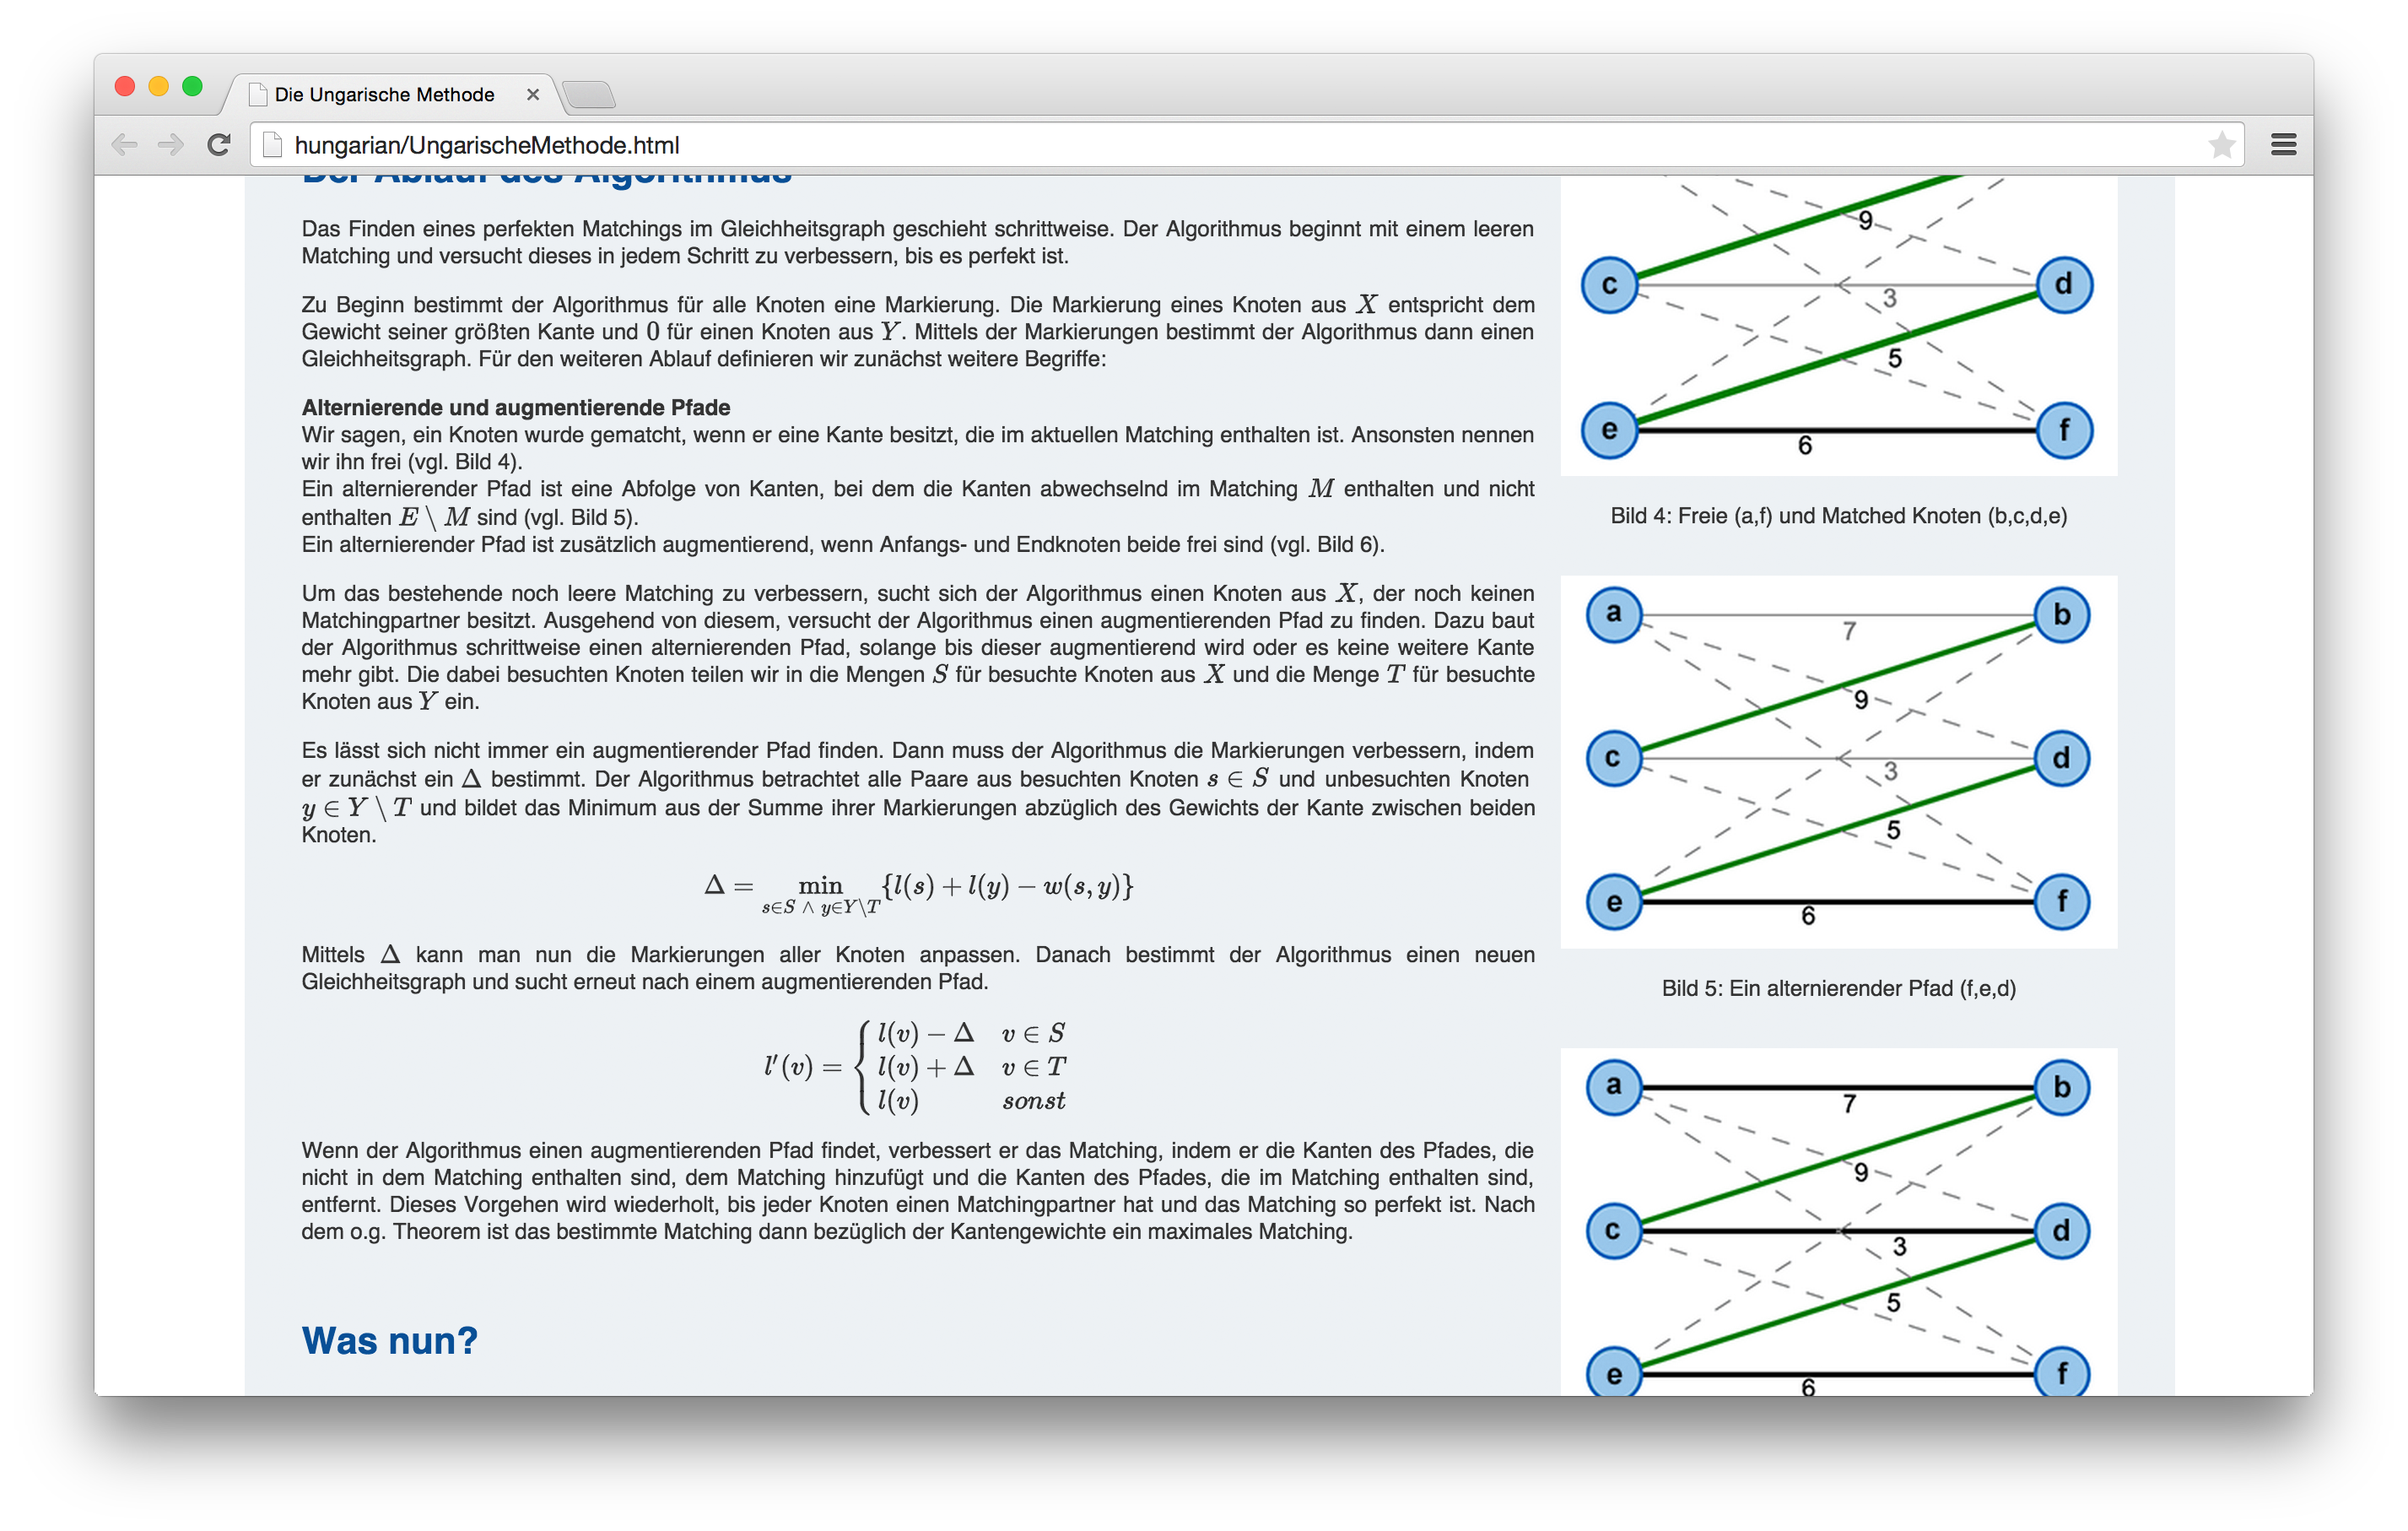
\includegraphics[width=\textwidth]{figures/mathjax-example}
	\caption[MathJAX Beispiel Browser]{MathJAX Beispiel: Darstellung im Browser}\label{fig:mathjax-example-img}
\end{figure}

Werden Ausdrücke zur Laufzeit in das DOM mittels JavaScript eingefügt, so müssen diese separat übersetzt werden (vgl. Abbildung~\ref{fig:listing-mathjax-render}).

\begin{figure}[h!]
\begin{lstlisting}[language=JavaScript]
MathJax.Hub.Queue(["Typeset", MathJax.Hub]);
\end{lstlisting}
\caption[MathJAX Render Befehl]{Befehl zum erneuten Rendern von Ausdrücken im HTML Dokument}\label{fig:listing-mathjax-render}
\end{figure}

\section{Bipartite Graphen}
Zwei Algorithmen, die im Rahmen des Projekts implementiert wurden, nämlich Hopcroft \& Karp Algorithmus und die Ungarische Methode, müssen auf bipartiten Graphen ausgeführt werden. Dafür haben wir das Konzept des bipartiten Graphen im existierenden Framework entwickelt. Um die Darstellung des Matching-Problems und dessen Lösung möglichst anschaulich zu machen, haben wir die Knoten im Graphen in zwei Gruppen geteilt (vgl. Abbildung~\ref{fig:hungarian-bipartite}). Die Kanten können nur zwischen den Knotengruppen erstellt werden. Bei der Ungarischen Methode war es wichtig den Graph mit extra Knoten und Kanten zu vervollständigen, wenn der ursprüngliche Graph nicht komplett war. Das ist notwendig, weil die Ungarische Methode perfektes Matching sucht.
\begin{figure}[h!]
	\centering
	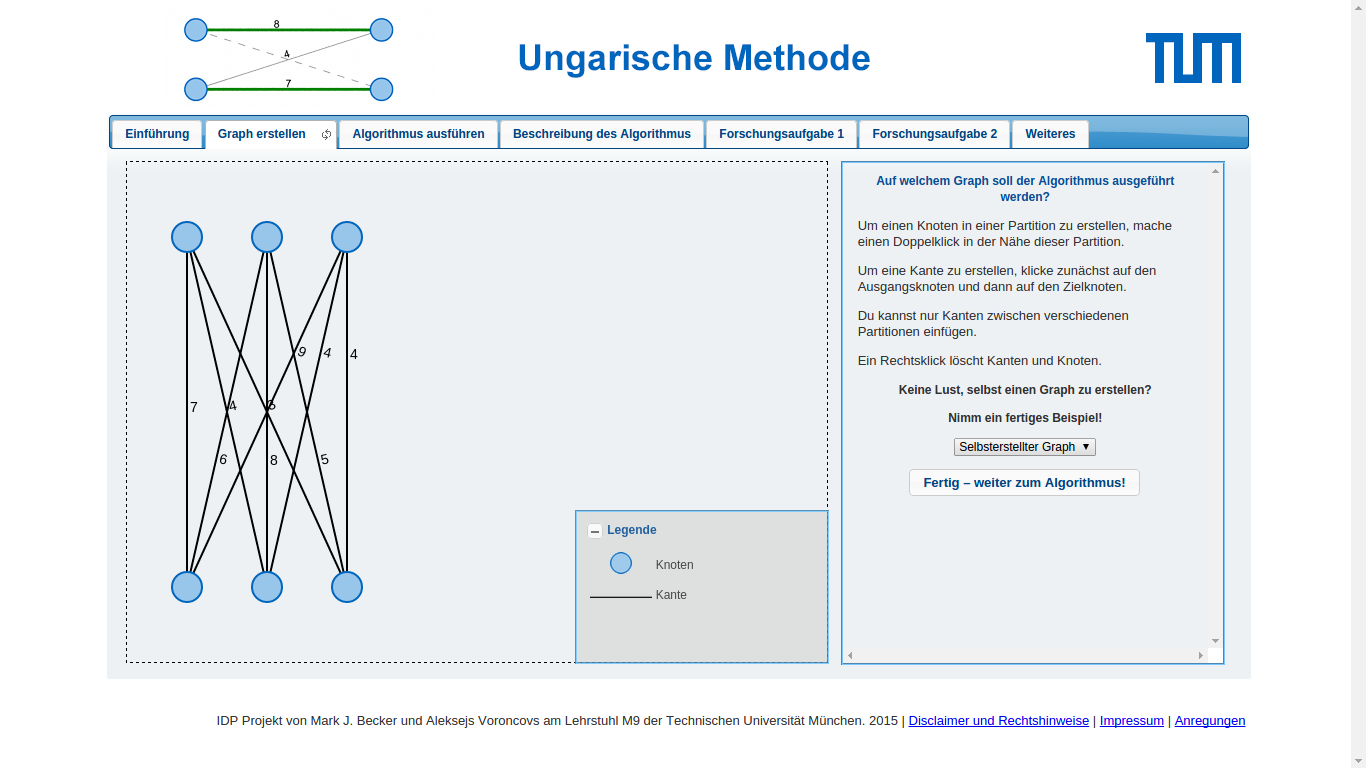
\includegraphics[width=\textwidth]{figures/hungarian-bipartite}
	\caption[Ungarische Methode]{Bipartiter Graph}\label{fig:hungarian-bipartite}
\end{figure}

In der Abbildung~\ref{fig:hungarian-complete} kann man sehen, was passiert, wenn man bei der Ungarischen Methode einen nicht kompletten Graphen eingibt. Falls eine Kante zwischen beliebigen zwei Knoten fehlt, wird eine zusätzliche graue Kante mit dem Gewicht 0 hinzugefügt. Wenn die Knotengruppen ungleiche Anzahl der Knoten enthalten, dann werden zusätzliche Knoten dem Graphen hinzugefügt. Alle Nachbarkanten bei diesen zusätzlichen Knoten haben das Gewicht 0.
\begin{figure}[h!]
	\centering
	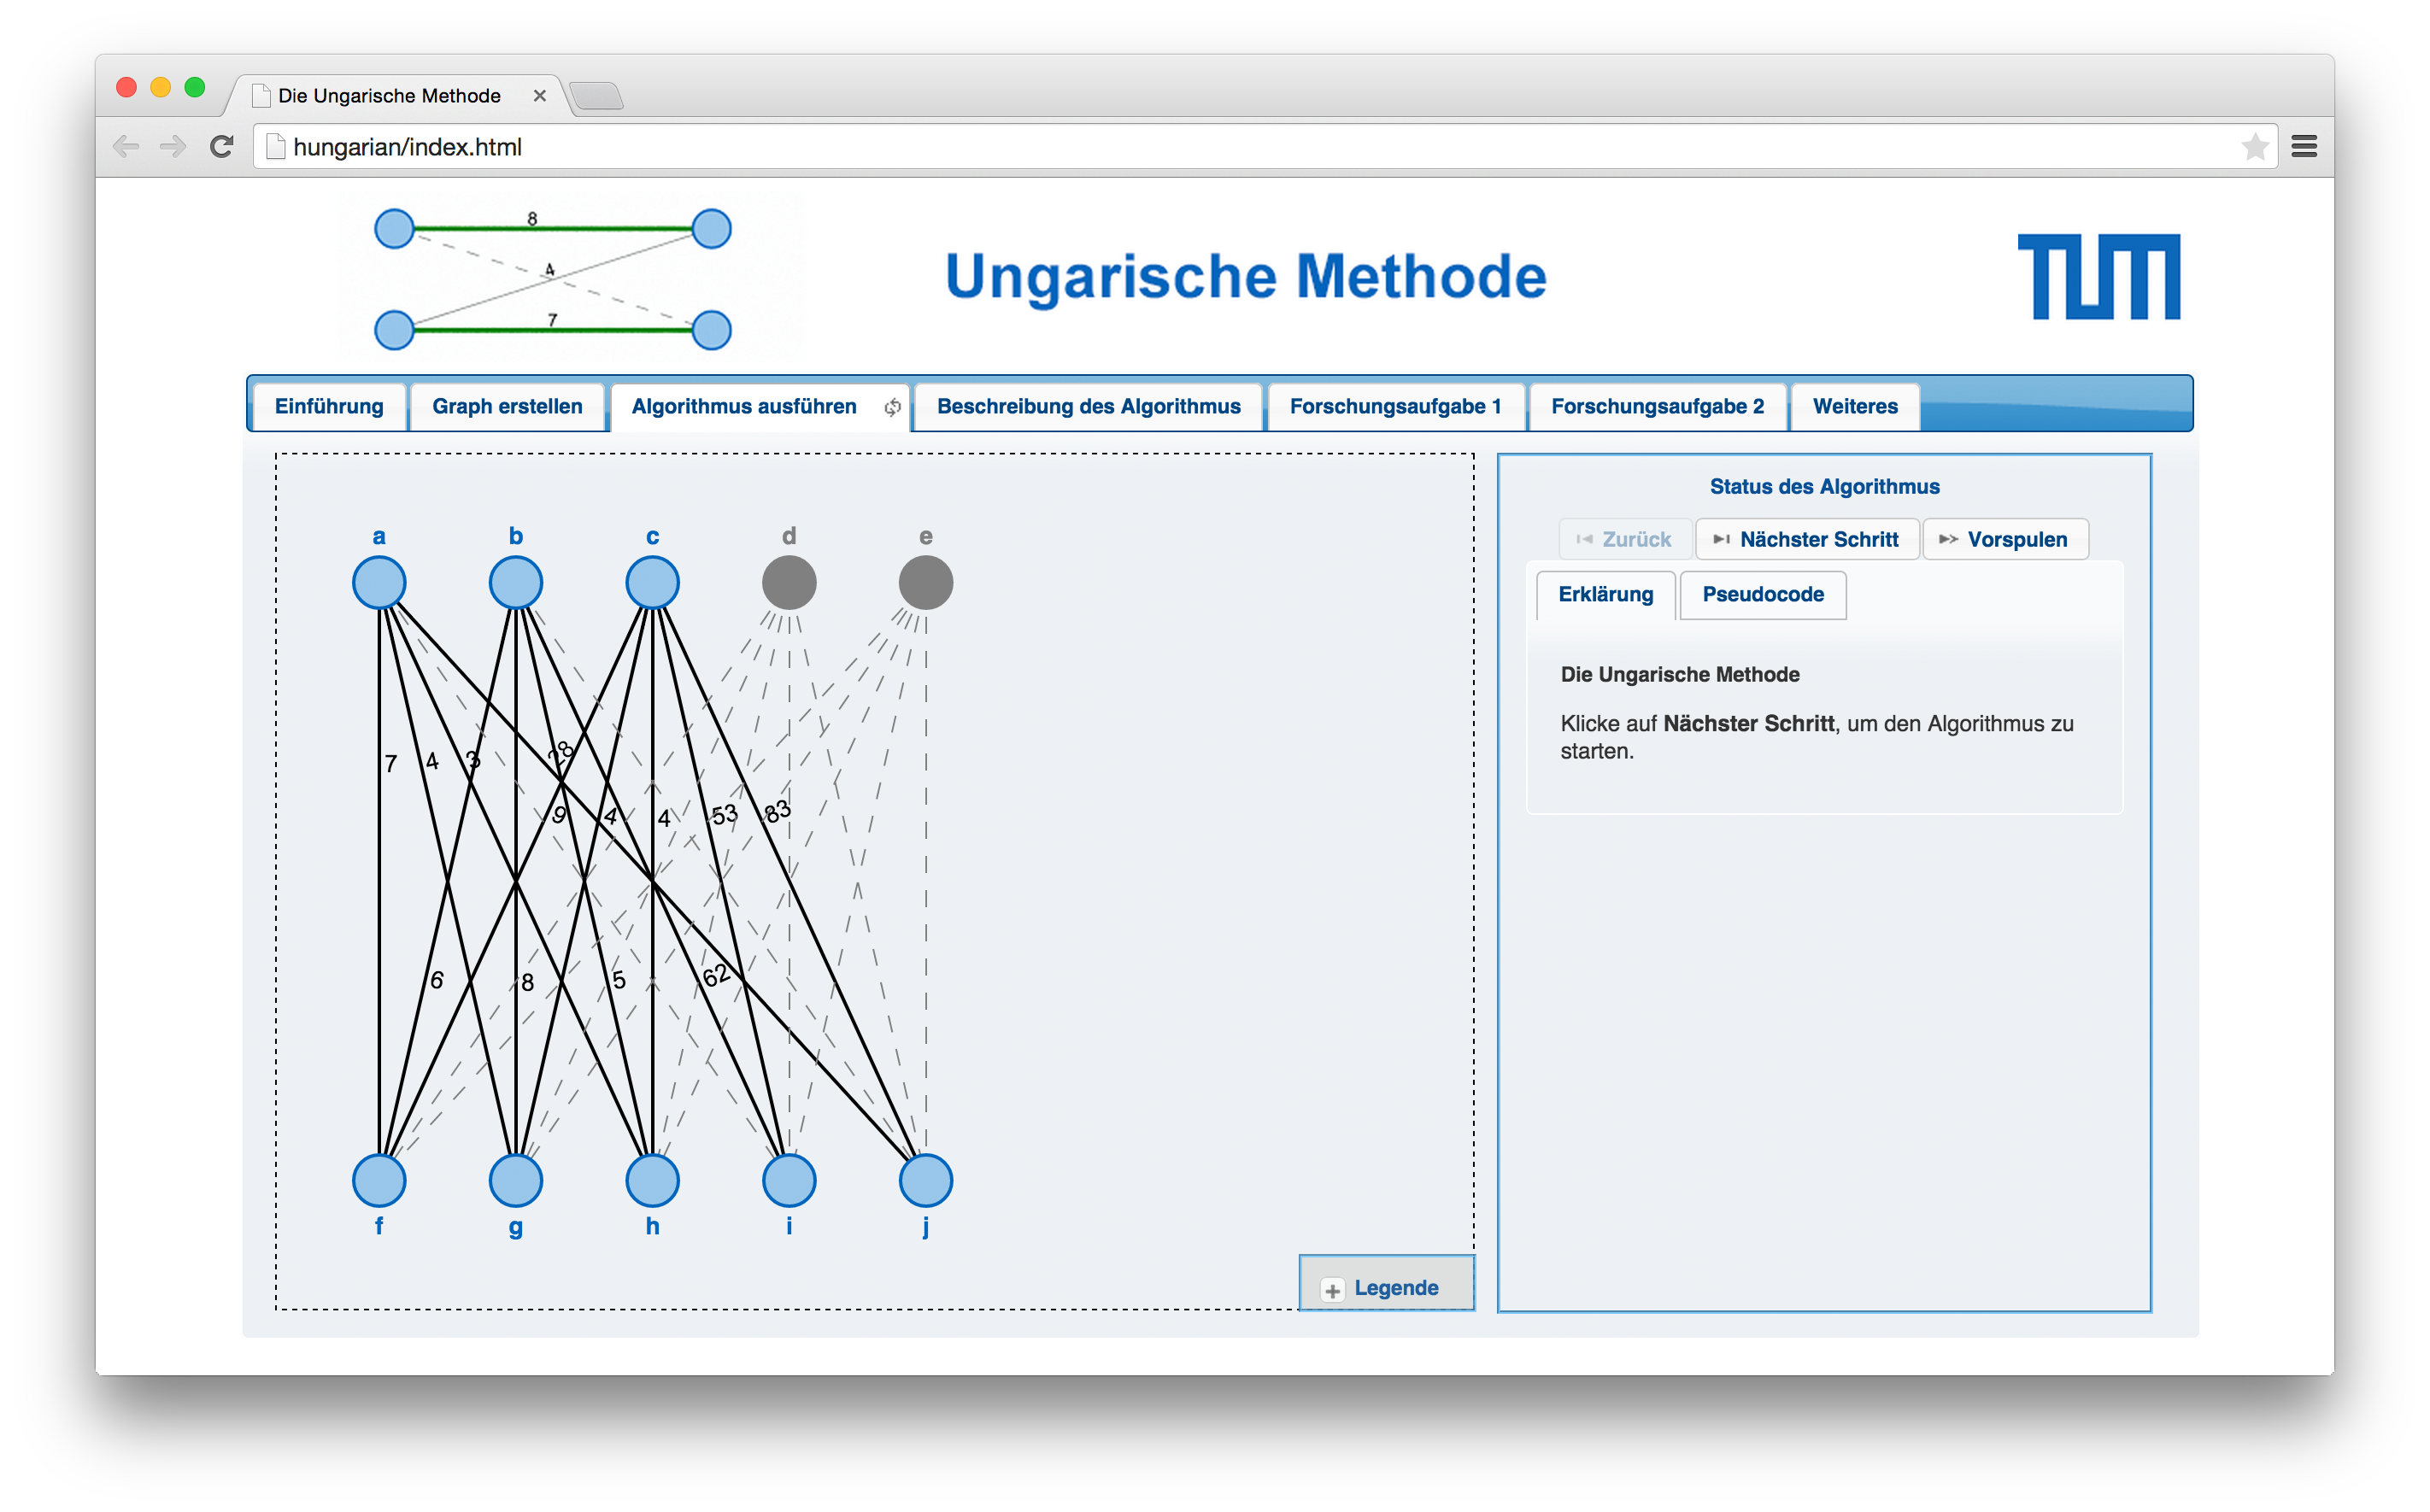
\includegraphics[width=\textwidth]{figures/hungarian-complete}
	\caption[Ungarische Methode]{Der Graph wird mit fehlenden Knoten und Kanten erweitert}\label{fig:hungarian-complete}
\end{figure}

\section{Multigraphen}
Motivation
Beispiel

\section{Zufällig generierte Fragen (Mark)}
In bisherigen auf diesem Framework basierenden Projekten war die Varianz der Fragen in den Forschungsaufgaben problematisch. Die Forschungsaufgaben behandelten meistens statische Fragen an vorher festgelegten Stellen zu vorgegebenen Graphen. Daraus resultierend bietet sich dem Nutzer ein wenig abwechslungsreiches Erlebnis und die Motivation, eine Forschungsaufgabe mehrfach zu bearbeiten, ist nicht gegeben.

In unserer Implementierung verfolgen wir daher einen anderen Ansatz. Die Forschungsaufgaben sind grundsätzlich so aufgebaut, dass sie die gleiche Struktur und den gleichen Quellcode wie die reguläre Ausführung des Algorithmus benutzen. Das schließt auch den vom Nutzer selbst gewählten Graph aus dem \enquote{Graph erstellen} Tab mit ein. Statt statischen Fragen definiert der Entwickler eine Menge von Fragetypen. Vor jedem Schritt des Algorithmus wird dann anhand einer Wahrscheinlichkeitsmatrix bestimmt, ob zu dem folgenden Schritt eine Frage gestellt wird und wenn ja, welcher Fragetyp gewählt werden soll. Außerdem sollen wenn möglich die Inhalte der generierten Fragen eines Fragetyps variieren. So werden beispielsweise die Knoten, zu denen ein Wert bestimmt werden soll, zufällig gewählt (vgl. Abbildung~\ref{fig:random-question}).

Mit dieser Implementierung gelingt es, dass in jeder Bearbeitung einer Forschungsaufgabe unterschiedliche Kombinationen von Fragen gestellt werden. Zusätzlich kann der Nutzer durch selbst erstelle Graphen auch Spezialfälle testen.

\begin{figure}[h!]
	\centering
	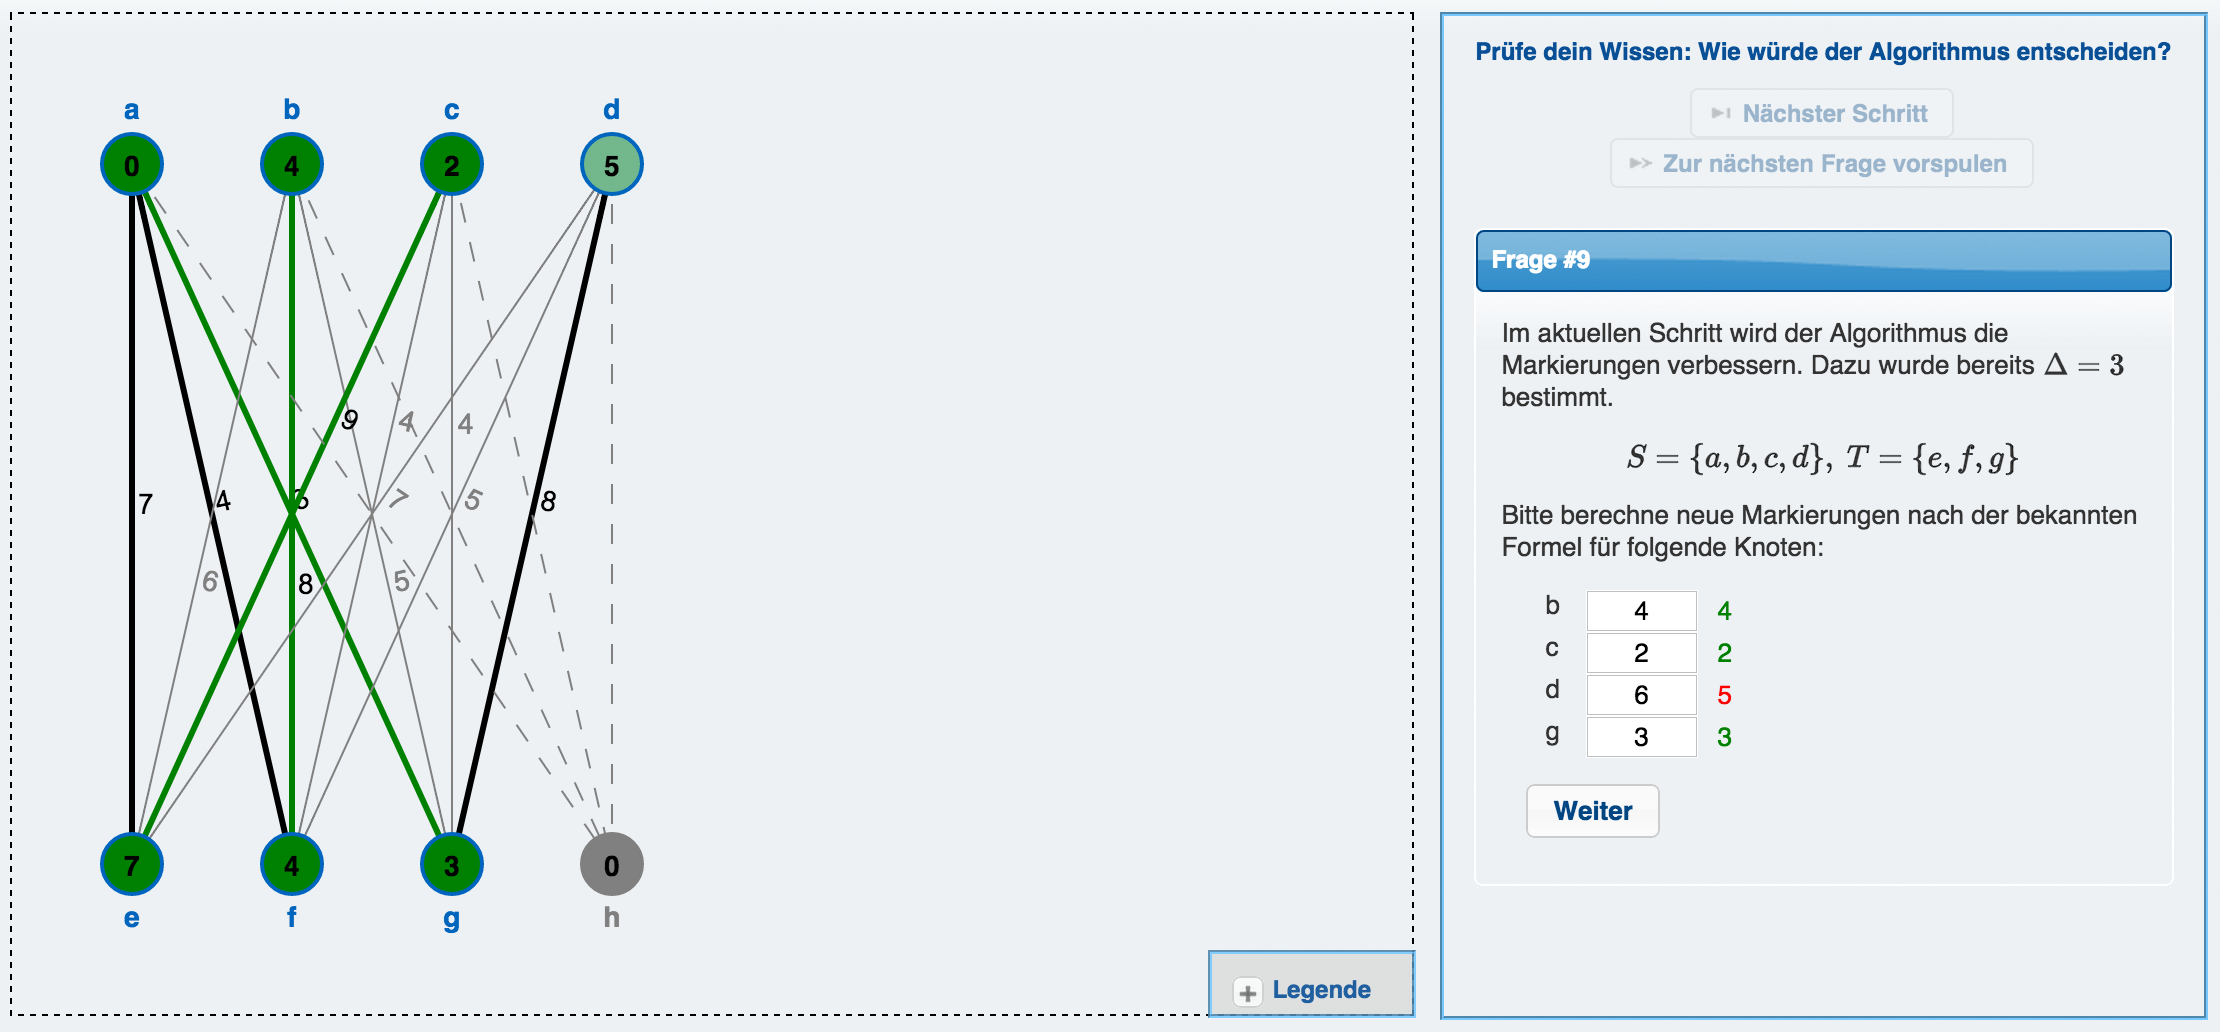
\includegraphics[width=\textwidth]{figures/random_question}
	\caption[Zufällig generierte Frage]{Beispiel für eine zufällig generierte Frage}\label{fig:random-question}
\end{figure}

\subsection*{Implementierung}
In der Funktion \texttt{this.nextStepChoice} wird vor der Auswahl des nächsten Schritts des Algorithmus mittels der Funktion \texttt{this.askQuestion} bestimmt, ob und welche Frage gestellt werden soll. Für jeden Fragetyp exisiert eine separate Funktion (bspw. \texttt{this.generateNextStepQuestion}), die auf den aktuellen Graph zugreift und eine Frage mit zufälligen Elementen generiert und in das DOM Element \texttt{\#tf1\_div\_questionModal} schreibt. Die gegebene Antwort wird durch Aufruf der Funktion \texttt{this.saveAnswer} gespeichert und mit der richtigen Lösung verglichen. Am Ende der Forschungsaufgabe kann mittels \texttt{this.showQuestionResults} eine Übersicht angezeigt werden, die zeigt, wieviele Fragen richtig beantwortet wurden. Weitere Informationen sind der Inline-Dokumentation zu entnehmen.

\section{Gemeinsam genutzte Dateien (Mark)}
Im Rahmen dieses interdisziplinären Projekts wurden Webapplikationen für insgesamt fünf Algorithmen entwickelt. Jede Applikation liegt in einem von den anderen Algorithmen unabhängigen Projektordner, der jeweils auch das Graph Framework aus früheren Projekten enthält. Daher lagen im gesamten Repository viele Dateien mehrfach vor. Dies war insofern problematisch, da Änderungen, die alle Anwendungen betreffen in mehreren Dateien vorgenommen werden mussten.

Unser Ziel war es daher, gemeinsam genutzte Dateien auszulagern. Wir beschränken uns hier auf Dateien, welche das Layout und Design der Anwendungen definieren sowie universelle Programmbibliotheken (bspw. MathJAX). Diese Beschränkung ist notwendig, um die Flexibilität im Entwicklungsprozess zu gewährleisten. Es existieren weitere Dateien, die sich zum aktuellen Zeitpunkt anwendungsübergreifend nicht signifikant unterscheiden. Diese sind allerdings algorithmenspezifisch und könnten in zukünftigen Entwicklungsphasen weiter verändert werden.

Zur Auslagerung legten wir zunächst einen \texttt{library} Ordner an. Das Finden von Dateiduplikaten übernimmt ein Python Skript (vgl. \texttt{deduplicate.py}), welches mittels der \texttt{difflib} Bibliothek alle Dateien in den Projektordnern paarweise miteinander vergleicht und einen Ähnlichkeitsquotienten bestimmt. Das Skript zeigt dann alle Dateien, die einen festgelegten Änhlichkeitsgrenzwert überschreiten an (vgl. Abbildungen \ref{fig:shared-files-1} und \ref{fig:shared-files-2}). Anhand des Quotienten lässt sich ablesen, ob Dateien im Gesamten oder in Teilen ausgelagert werden können. Das Verschieben in den \texttt{library} Ordner und die Anpassung der Pfade in den Anwendungen erfolgt dann manuell.

\begin{figure}[h!]
\noindent\texttt{chinese-postman/img/TUMLogo.png \\
-> 100.00\% identical to floyd-warshall/img/TUMLogo.png \\
-> 100.00\% identical to hierholzer/img/TUMLogo.png \\
-> 100.00\% identical to hopcroft-karp/img/TUMLogo.png \\
-> 100.00\% identical to hungarian/img/TUMLogo.png
}
\caption[Gemeinsame Dateien, Beispiel 1]{Vollständige Übereinstimmung bei der Datei \texttt{TUMLogo.png}}\label{fig:shared-files-1}
\end{figure}

\begin{figure}[h!]
\noindent\texttt{chinese-postman/js/siteAnimation.js \\
-> 67.01\% identical to hierholzer/js/siteAnimation.js \\
-> 91.49\% identical to hopcroft-karp/js/siteAnimation.js \\
-> 71.13\% identical to hungarian/js/siteAnimation.js
}
\caption[Gemeinsame Dateien, Beispiel 2]{Mäßige Übereinstimmungen bei der Datei \texttt{siteAnimation.js}}\label{fig:shared-files-2}
\end{figure}

Für zukünftige Projekte können die Parameter des Skripts angepasst werden. Weitere Informationen hierzu sind der Inline-Dokumentation zu entnehmen.

\chapter{Zusammenfassung}
Zusammenfassung der wesentlichen Punkte